\documentclass[12pt singlecol]{article}
% \usepackage{multicol,caption}
\usepackage[english]{babel}
%\usepackage{booktabs}
% \usepackage{float}
\usepackage{graphicx}
\DeclareGraphicsExtensions{.pdf,.png,.jpg}

% \usepackage{dblflfatfix}
% \newenvironment{Figure}
  % {\par\medskip\noindent\minipage{\linewidth}}
  % {\endminipage\par\medskip}

% 1 in Margfns
\usepackage[letterpaper]{geometry}
\geometry{top=1.0in, bottom=1.0in, left=1.0in, right=1.0in}

% Double Spacing
\usepackage{setspace}
\singlespacing

% Set font
\usepackage{times}

% Fancy-header package to modify header/page numbering
\usepackage{fancyhdr}
	\pagestyle{fancy}
	\fancypagestyle{plain}{\fancyhf{}}
		\lhead{\today}
		\chead{Laser Cutting}
		\rhead{\fancyplain{}{Vargas \thepage}}
		\lfoot{}
		\cfoot{}
		\rfoot{}
	\renewcommand{\headrulewidth}{0pt}
	\renewcommand{\footrulewidth}{0pt} 
	% To make sure we actually have header 0.5in away from top edge 
	% 12pt is one-sixth of an in. Subtract this from 0.5in to get headsep value
	\setlength\headsep{0.333in}

% Begin Document
\begin{document}

% Body of Paper
\title{Carving Out a Brighter Piece of Tomorrow:\\\emph{A Portrait Laser Cutting}}
\author{Patrick Vargas\\ATLS 3020: Digital Media 2\\Professor J. Harrim\\University of Colorado Boulder}
\date{\today}

\thispagestyle{plain}
\maketitle
% \newpage

\begin{flushleft}

% Change paragraph indentation to 0.5in
\setlength{\parindent}{0.5in}
\twocolumn
\section{What is laser cutting?}

If you don't know what laser cutting is, most likely seen the result of it. Artifacts of laser cutting have the look and feel something hand cut, but with a fine, sealed edge. Laser cutting can produce a range of artifacts. Eric Standly created beautiful artworks by layering pieces of laser cut paper. \cite{standley} See figures~\ref{fig:eric1},~\ref{fig:eric2},~\ref{fig:eric3}, and~\ref{fig:eric4}. Adam and April make a steady living off laser cut jewlery they make int thier studio in Tennessee. \cite{licketycut13} See figures~\ref{fig:birds},~\ref{fig:lcportal}, and~\ref{fig:lcplant}. Amanda Gahessaei pushes the medium of laser cutting forward with her wooden record. \cite{ghassaei13} See figures~\ref{fig:amanda1},~\ref{fig:amanda2}, and~\ref{fig:amanda3}. 

Laser cutting takes a high-energy laser and cuts through a piece of material. ``The material then melts, burns or vaporizes leaving an edge with a high-quality finish.'' \cite{Ponoko13} The material can be pretty much anything, but most common materials include wood, acrylic and steel. ``The laser beam is guided by lines on a vector file [\ldots]'' of whatever the design may be. \cite{Ponoko13} ``The laser works like a printer, so you can use most [\ldots] design software programs (such as CorelDRAW, Adobe products, or AutoCad.)'' \cite{Epilog09}.

\section{Where did laser cutting get it's start?}

Laser cutting's main element, the laser, is a good place to begin, theoretically. ``In 1917, physicist Albert Einstein theorized the principle of a laser, when he described his theory of stimulated emission.'' \cite{Morgan13} This lead to many engineers across the world to begin experimentations to create this ``Light Amplification by Stimulated Emission of Radiation'', or ``laser'' for short. \cite{LTI13} ``Theodore Maiman made the first laser operate on 16 May 1960 at the Hughes Research Laboratory in California, by shining a high-power flash lamp on a ruby rod with silver-coated surfaces.'' \cite{Townes03} 

Theodore Maiman later tried publishing his research in the \emph{Physical Review Letters} but was turned down. He then submitted to the paper, \emph{Nature} who published his paper on August 6th of that year.
\begin{quotation}
With official publication of Maiman's first laser under way, the Hughes Research Laboratory made the first public announcement to the news media on 7 July 1960. This created quite a stir, with front-page newspaper discussions of possible death rays, but also some skepticism among scientists, who were not yet able to see the careful and logically complete Nature paper. \cite{Townes03} 
\end{quotation}

\section{How is this achieved?}

Lasers are made by injecting energy into atoms, forcing them to give off protons.
\begin{quotation}
Lasers work by adding energy to atoms or molecules, so that there are more in a high-energy (``excited'') state than in some lower-energy state; this is known as a ``population inversion.'' When this occurs, light waves passing through the material stimulate more radiation from the excited states than they lose by absorption due to atoms or molecules in the lower state. \cite{Townes03}
\end{quotation}
From here, the photons are released by the electrons. These protons are then reflected off a mirror which causes other electrons to give off more protons. Figure~\ref{fig:how} details this process. ``The laser beam [used in laser cutting] is a column of very high intensity light, of a single wavelength, or color. In the case of a typical [carbon dioxide] laser, that wavelength is in the Infra-Red part of the light spectrum, so it is invisible to the human eye. '' \cite{Zlotnicki13}

\begin{figure}
	\centering	
	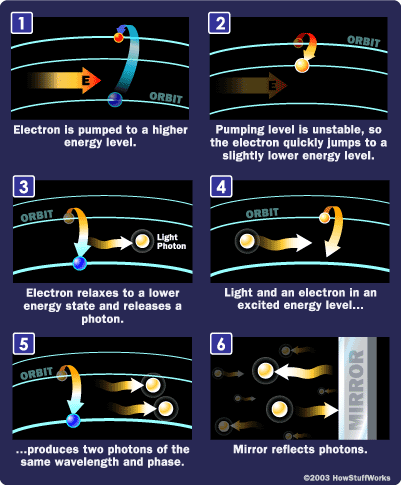
\includegraphics[width=\linewidth]{laserhow}
	\caption{Recapitulation of how a laser works. \cite{Weschler00}}
	\label{fig:how}
\end{figure}

The process of laser cutting enhances the laser and refines the beam onto the surface of the material. Most commonly, carbon dioxide is the chemical found in the laser. To refine the beam, a series of mirrors are used as well as a gas, most commonly oxygen or nitrogen. ``The great interest in carbon dioxide lasers stems from their continuous power capability, high efficiency and ease of construction.'' \cite{WhitehouseND} Carbon dioxide lasers typically have a power density of 60-80 Watts per meter, with a maximum output capacity of 1200 Watts, giving this type of laser a power efficiency rating of 15\%-20\%. Compare that with helium-neon lasers and argon lasers which both have a power efficiency rating of 0.1\%, Carbon dioxide lasers are the clear choice. \cite{WhitehouseND}
\begin{quotation}
The beam, [in carbon dioxide lasers are] only about 3/4 of an inch in diameter as it travels from the laser resonator, which creates the beam, through the machine's beam path. It may be bounced in different directions by a number of mirrors, or ``beam benders'', before it is finally focused onto the plate. The focused laser beam goes through the bore of a nozzle right before it hits the plate. Also flowing through that nozzle bore is a compressed gas, such as Oxygen or Nitrogen. \cite{Zlotnicki13}
\end{quotation}
See Figure~\ref{fig:refract} for a graphical example of laser cutting. The use of oxygen and nitrogen in laser cutting is for different results. For example, ``[o]xygen is used as a cutting gas mainly for non-alloyed and low-alloyed steels. The jet of cutting gas oxidizes the material melted by the laser beam and blows away the melt and slag from the cutting groove.'' \cite{agao212} By using oxygen on metals, the oxidization process kicks in and assists the laser in cutting through thicker metals.

\begin{figure}
	\centering	
	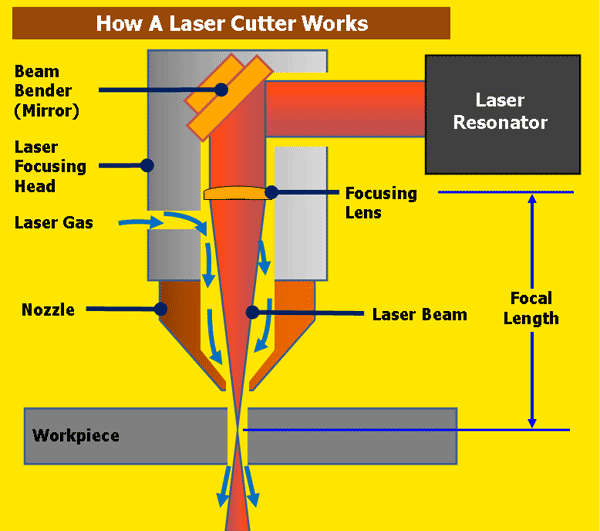
\includegraphics[width=\linewidth]{refract}
	\caption{Graphical representation of how a laser cutter works. \cite{Zlotnicki13}}
	\label{fig:refract}
\end{figure}

On the other hand, using nitrogen helps the laser to prevent the added heat oxidization provides. ``When nitrogen is used as the cutting gas, the laser beam melts the material, and the nitrogen blows away the molten material from the cutting groove. Since no exothermic reaction takes place, the cutting speed is much slower than when cutting with oxygen.'' \cite{agan12} Typically, laser cutting uses nitrogen with highly, combustible materials, such as wood, leather or paper. ``A combustible material [\ldots] must not [\ldots] be cut with oxygen, as the work-piece would catch fire. Oxygen should only be used for metallic work-pieces with oxide-free edges.'' \cite{esab13}

\section{How do designers make laser cut designs?}

Anyone can make a laser cut artifact with the help of vector-based design software. To print the design, an artist can either purchase their own laser cutter or have a production company print the design for them, for a fee. Most laser cutters not used industrially cost anywhere between \$1,800 and \$10,000. \cite{fsl11} 

Numerous companies provide a much cheaper option for designers, such as Ponoko, 100kGarages, and Pololu. These shops generally have a price per minute pricing scheme. What this means is a designer is charged per minute the machine is taking cutting the design. Therefore, the more intricate the pattern, the more expensive the result will be. \cite{PonokoPrice13,garages12,pololu12}

Many options are available for vector-based design software. Notable products include Adobe Illustrator (\$19.99/month), CorelDRAW (\$399.00), and Inkscape (Free). \cite{adobe13,corel13,inkscape13} The overall size a design can be depends on the size of the machine. For example, at Ponoko, the largest design must be less than 31.1 inches by 15.1 inches. \cite{PonokoStarter13} 

\begin{figure}
  \centering  
  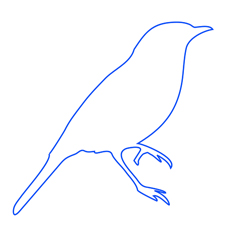
\includegraphics[width=\linewidth]{cutting-line}
  \caption{What the laser cutter cuts along. \cite{PonokoStarter13}}
  \label{fig:cutline}
\end{figure}

\begin{figure}
  \centering  
  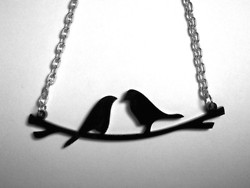
\includegraphics[width=\linewidth]{cut-birds}
  \caption{What is produced by cutting. ``Little Birds Laser Cut Acrylic Charm Necklace'' by LickityCut \cite{licketycut13}}
  \label{fig:birds}
\end{figure}	

Laser cutters follow lines on a vector file and will produce different results depending on the color. For example, if you want to cut out a shape, the laser cutter would follow a solid blue line (rgb(0, 0, 255)) at 100\% opacity in the alpha channel. \cite{PonokoStarter13} See figure~\ref{fig:cutline}  for the vector example and figure~\ref{fig:birds} for the result of the cutting technique. When an artist designs for a piece to be cut, they need to make sure to account for the size of the material being cut with respect to the size of the laser. For example, if the material is 2 mm thick, the laser will cute lines that are 1.4 mm wide. If the material is 12 mm thick, then the laser will cut lines that are 2.5 mm wide. In other words, the thicker the material, the wide the cut line will be. \cite{agan12}

\begin{figure}
  \centering  
  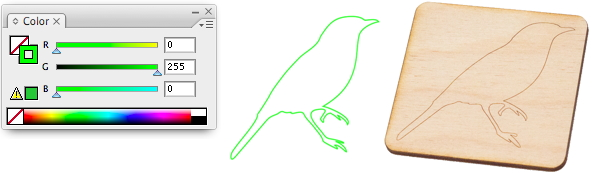
\includegraphics[width=\linewidth]{engrave}
  \caption{Defining the engraving line. \cite{PonokoAdvance13}}
  \label{fig:engrave}
\end{figure}	

\begin{figure}
  \centering  
  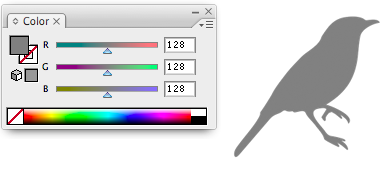
\includegraphics[width=\linewidth]{fill}
  \caption{Defining the engraving fill areas. \cite{PonokoAdvance13}}
  \label{fig:fill}
\end{figure}	

Laser cutters are also able to engrave a piece. What this means is the laser only goes through part of the material, not all the way through. This can add depth to a piece of work. Engraving can either be engraved lines or filled areas. For example, the vector file would draw a solid red (rgb(255, 0, 0)), green (rgb(0, 255, 0)), or magenta (rgb(255, 255, 255)) line depending on depth desired. See figure~\ref{fig:engrave} for an example. If a fill is desired, the vector fill would block out sections in varying degrees of gray, ranging from deepest depth, black (rgb(0, 0, 0)), to no depth, white (rgb(255, 255, 255)). As long as the values of R.G.B. are equal, an artist can designate any depth they require. See figure~\ref{fig:fill} for an example.

\section{What is the result of all of this?}

There are numerous artists and hobbyists out there that make use of laser cutting. They design using software and materials, and combine them in interesting ways. They then can sell the manufactured products, usually online through their own sites of craft sites such as Etsy, and make a good side business. \cite{etsy13}

\subsection{Case Study: Eric Standley}

Eric Standley is a professor of art in the School of Visual arts at Virginia Tech in Virgina. He got a bachelors of fine art from the Massachusetts College of Art. Eric later got his masters of fine art from the Savannah College of Art and Design. Eric, ``dreams that with hard work and concentration he might one day become a modernist. He holds allegiance to a faith of his own construction, which is reinvented on a daily basis.'' \cite{standley} 

\begin{figure}
  \centering  
  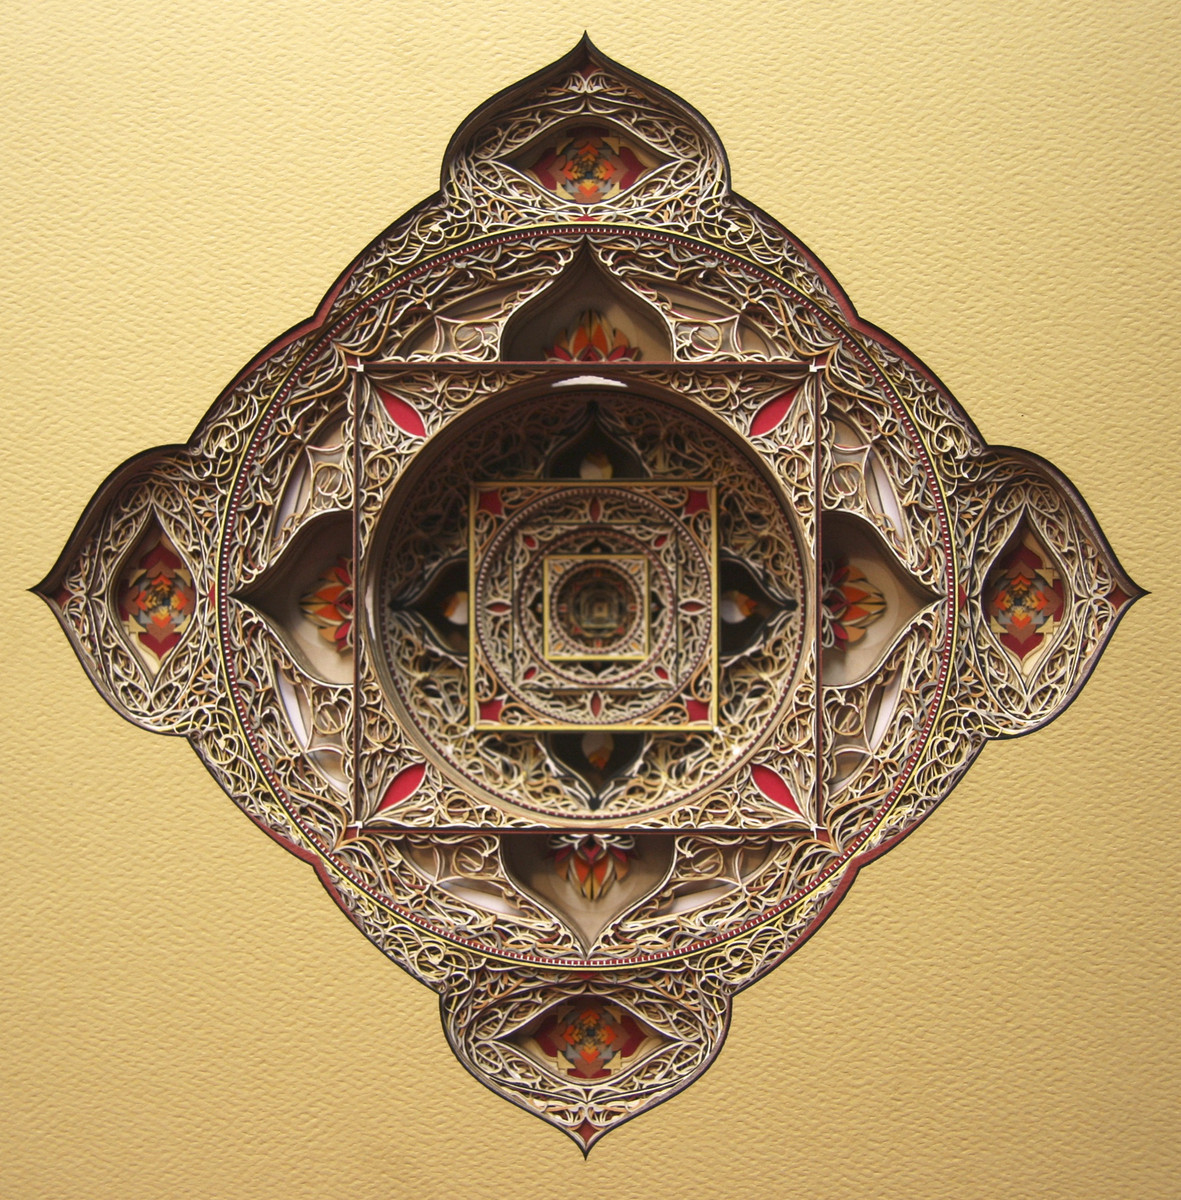
\includegraphics[width=\linewidth]{eric1}
  \caption{``Zeno of Elea'' by Eric Standley \cite{standley}}
  \label{fig:eric1}
\end{figure}	

\begin{figure}
  \centering  
  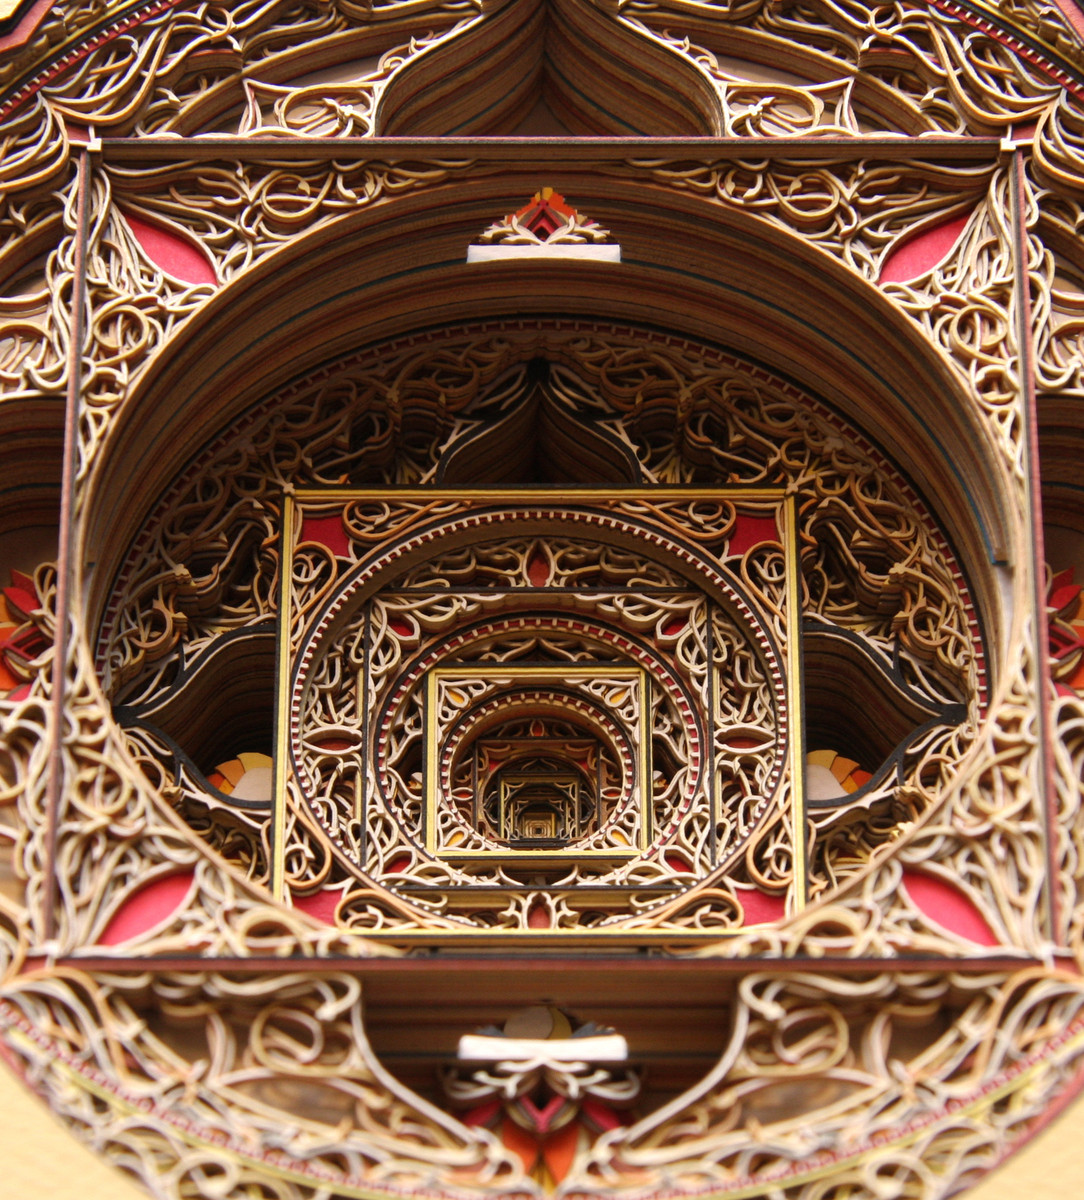
\includegraphics[width=\linewidth]{eric2}
  \caption{``Zeno of Elea'' (detail) by Eric Standley \cite{standley}}
  \label{fig:eric2}
\end{figure}	

Eric first draws out his design on paper. He then figures out the best way to combine the positive and negative spaces to create a three-dimensional effect. Eric then cuts individual pieces of paper using a laser cutter and then places them one on top of the other to create the pieces found in figures~\ref{fig:eric1},~\ref{fig:eric2},~\ref{fig:eric3}, and~\ref{fig:eric4}. \cite{standley, david13}

\begin{figure}
  \centering  
  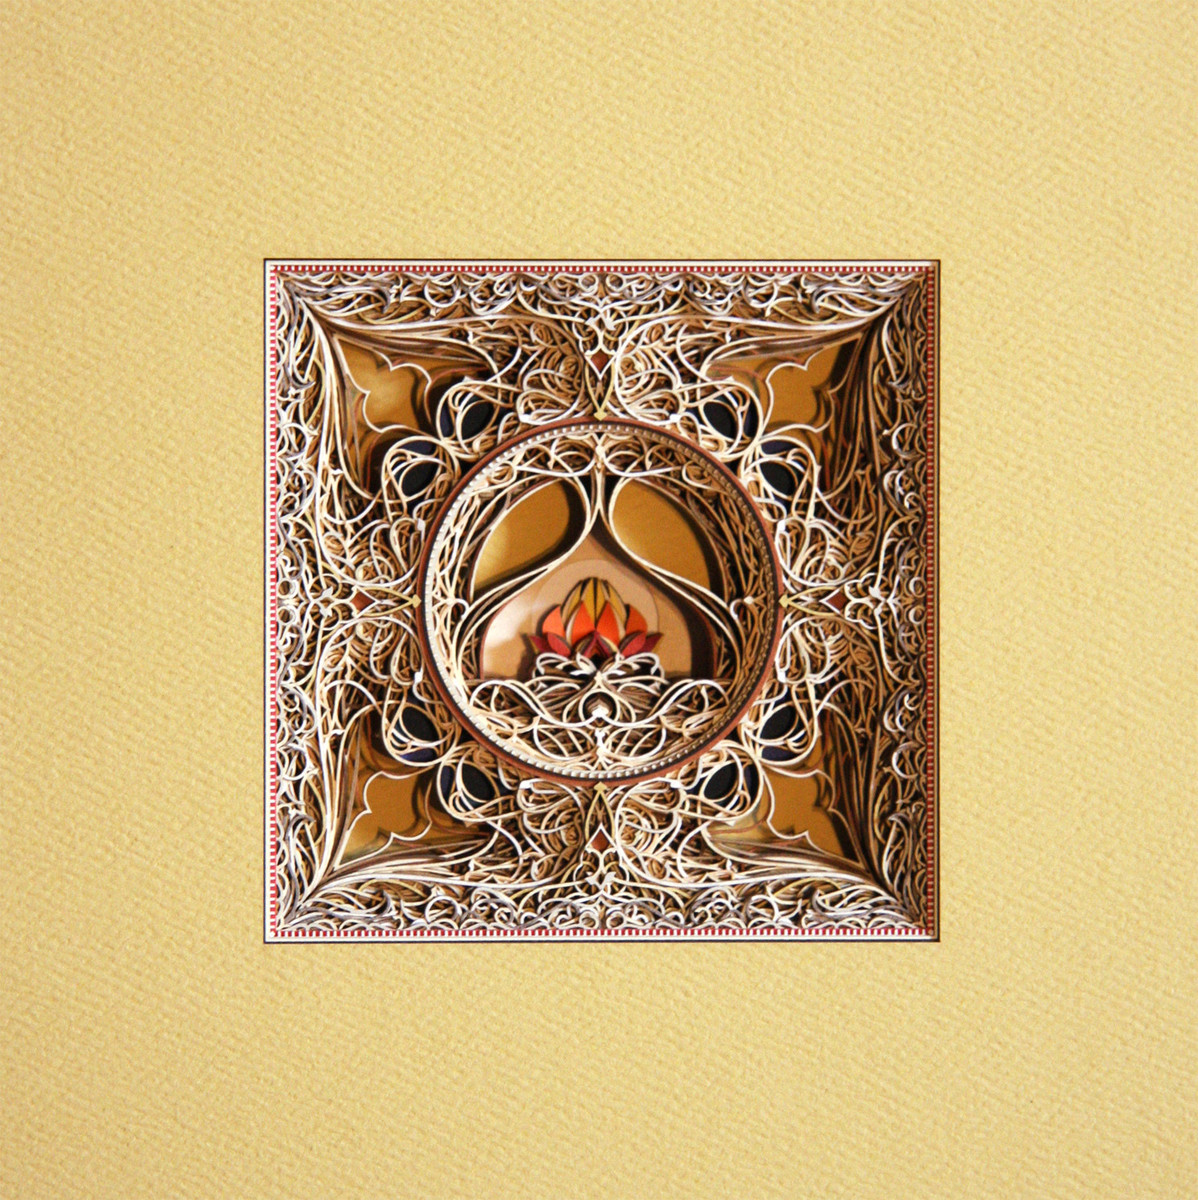
\includegraphics[width=\linewidth]{eric3}
  \caption{``Either/Or Circle 4.14.1'' by Eric Standley \cite{standley}}
  \label{fig:eric3}
\end{figure}	

\begin{figure}
  \centering  
  
\includegraphics[width=\linewidth]{eric4}
  \caption{``Either/Or Circle 4.14.1'' (detail) by Eric Standley \cite{standley}}
  \label{fig:eric4}
\end{figure}	

\subsection{Case Study: LickityCut}

LickityCut is a couple in Tennessee who make acrylic jewelery. The couple, Adam and April, originally sold their designs through Etsy and have been in production since 2009. They recently decided to switch to their own site to sell their products. See figures~\ref{fig:birds},~\ref{fig:lcportal}, and~\ref{fig:lcplant} for example of their work.

\begin{figure}
  \centering  
  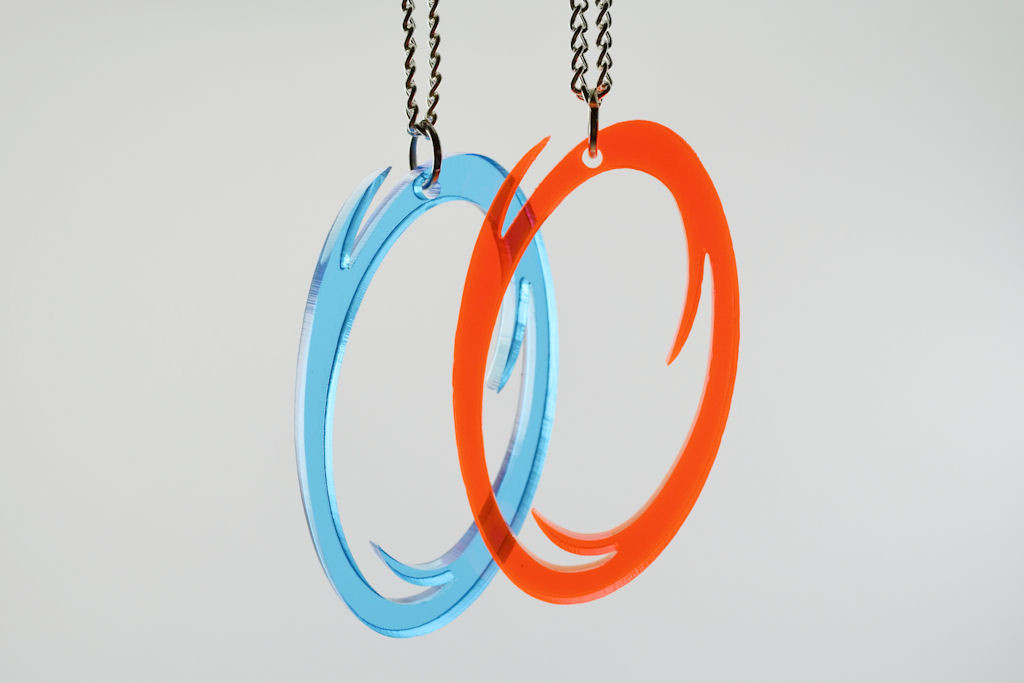
\includegraphics[width=\linewidth]{lcportal}
  \caption{``Portal Friendship Necklaces - Orange and Blue Portal Necklaces- GLaDOS'' by LicketyCut \cite{licketycut13}}
  \label{fig:lcportal}
\end{figure}	

\begin{figure}
  \centering  
  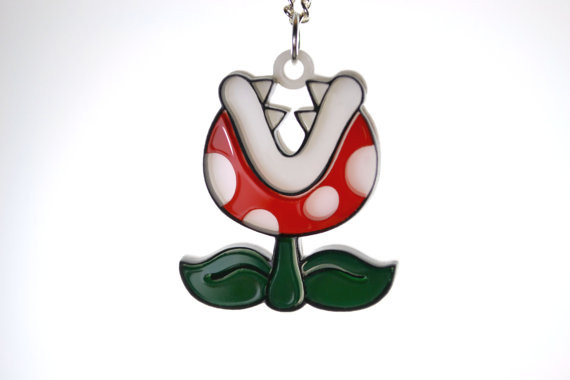
\includegraphics[width=\linewidth]{lcplant}
  \caption{``Piranha Plant Laser Cut Acrylic Gaming Necklace'' by LicketyCut \cite{licketycut13}}
  \label{fig:lcplant}
\end{figure}	

\subsection{Case Study: Amanda Ghassaei}

Amanda Ghassaei got a bachelors of art in physics with a minor in chemistry in 2011 from Pomona College in Claremont, California. As a professional scientist, Amanda's research experiences includes nano-technology, solar cells, and electrochemical and optical sensors. Her interests include, novel applications of digital fabrication, materials science, and developing physical interfaces for the manipulation of digital media. She currently resides in San Francisco and works for Instructables.com \cite{ghassaei13}

In 2013, Amanda laser cut a record out of a block of wood. She wrote a program in Processing which allowed her to input a song file and get the resulting vector file. She then fed the vector file into an Epilog 120 Watt Legend EXT laser cutter. ``The audio on the records has a bit depth between 4-5 bit and a sampling rate up to about 4.5kHz.'' \cite{EpilogMain09, processing13, ghassaei13} 

\begin{figure}
  \centering  
  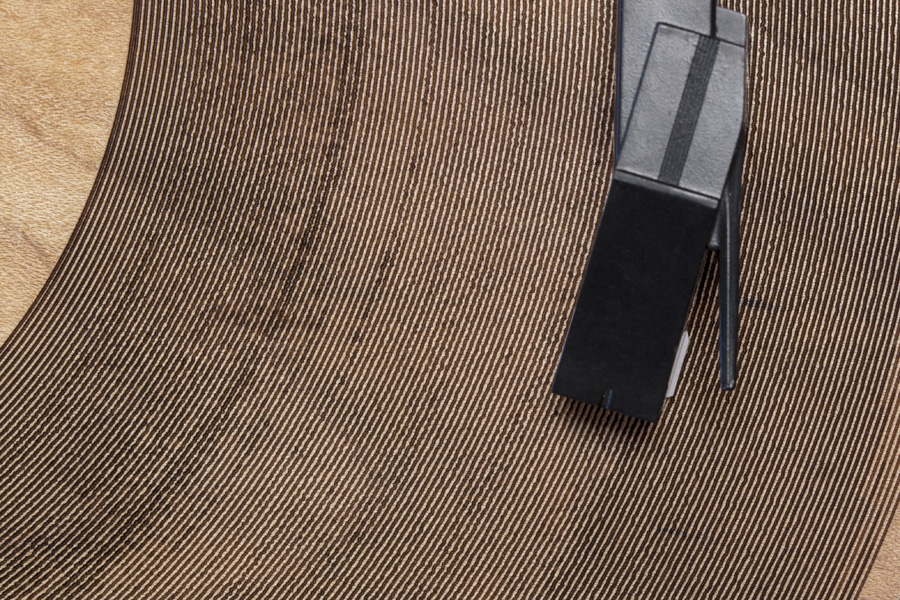
\includegraphics[width=\linewidth]{amanda1}
  \caption{``Laser Cut Record'' by Amanda Ghassaei \cite{ghassaei13}}
  \label{fig:amanda1}
\end{figure}	

``Processing is a programming language, development environment, and online community.'' \cite{processing13} Processing is open source and under the Creative Commons license. Through processing, an artist can create interactive programs which can be output with two-dimensional, three-dimensional or PDf capabilities. Amanda wrote her processing sketch, as the programs are called, ``that generates the record cutting paths so that [the sketch] can be modified for any song, material, cutting machine, record size, and turntable speed.'' \cite{instruct13}

\begin{figure}
  \centering  
  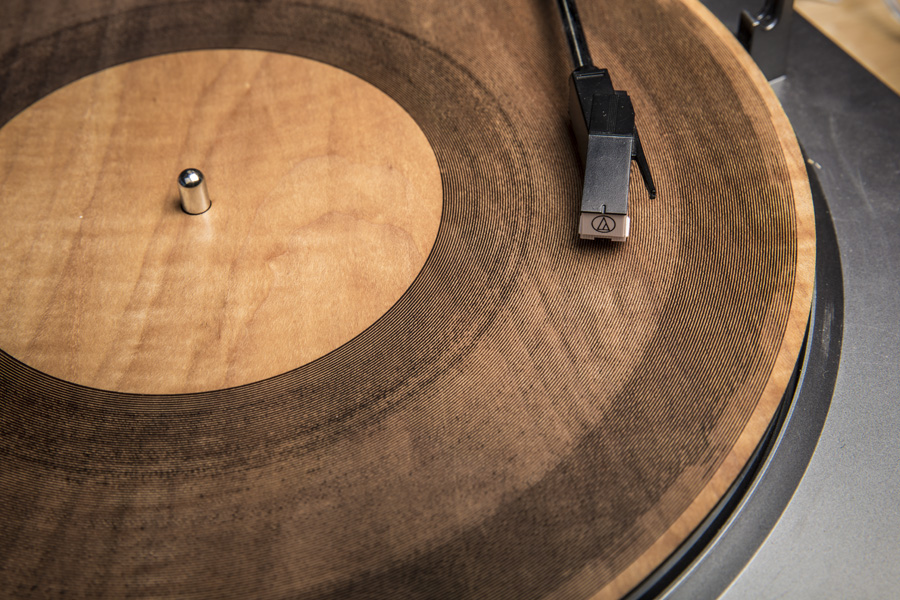
\includegraphics[width=\linewidth]{amanda2}
  \caption{``Laser Cut Record'' by Amanda Ghassaei \cite{ghassaei13}}
  \label{fig:amanda2}
\end{figure}

To create the record, Amanda first took her song file and equalized the song in a program called Audacity. \cite{instruct13, audacity}. She then wrote a python script that translated her song file into a text file. \cite{instruct13, python}. Amanda then fed the text file into her processing program, which then output a vector-design as a pdf file. \cite{instruct13, processing13} Amanda works for Instructables, so anyone can download her code and make their own records. \cite{instruct13} See figures~\ref{fig:amanda1},~\ref{fig:amanda2}, and~\ref{fig:amanda3} for pictures of the records created, which are an example of engraving.

\begin{figure}
  \centering  
  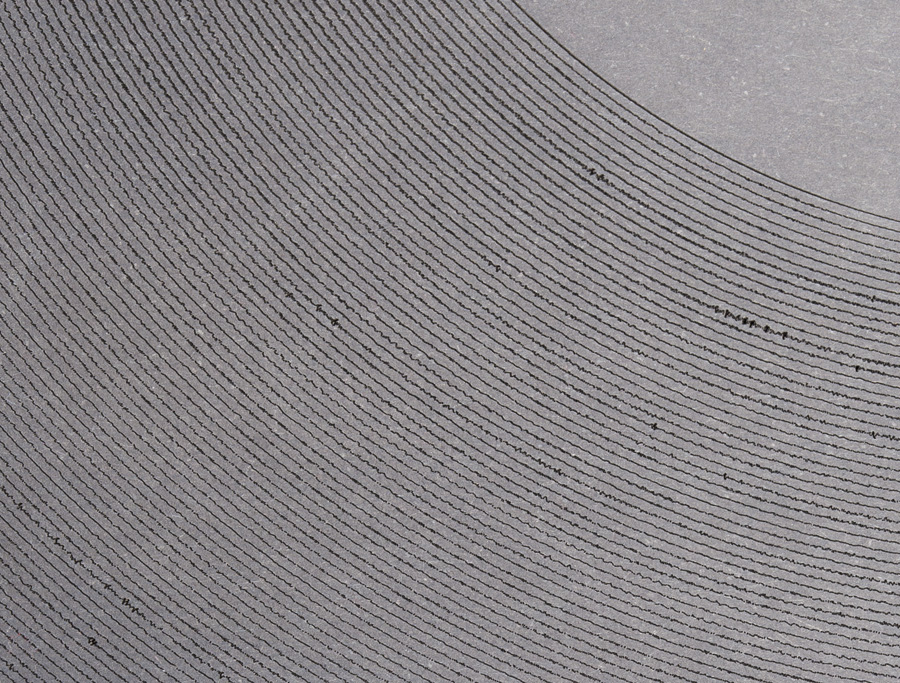
\includegraphics[width=\linewidth]{amanda3}
  \caption{``Laser Cut Record'' by Amanda Ghassaei \cite{ghassaei13}}
  \label{fig:amanda3}
\end{figure}	

\section{Conclusion}

Laser cutting is a fascinating medium of choice for many artists, designers and hobbyists. By harnessing the power of science, a laser can be refined to cut and engrave many materials. These materials can then be combined to create stunning pieces of work. You can be an artist like Eric Standly who dreams of becoming a modernist. \cite{standley} Or you can be a couple like Adam and April who make a living off of the inspiration of video games, science fiction and television. \cite{licketycut13} Or you can be a scientist like Amanda Ghassaei who pushes the medium forward for the sake of science. \cite{ghassaei13} The possibilities are endless in the medium of laser cutting. With it's humble beginnings, laser cutting sure has grown into it's own as a fascinating tool for art, design, and the pursuit of beauty.

% Works Cited
\newpage % This is needed if the book class is used, to place the anchor in the correct page,
         % because the bibliography will start on its own page.
         % Use \clearpage instead if the document class uses the "oneside" argument
\renewcommand*{\refname}{} % This will define heading of bibliography to be empty, so you can...
\onecolumn
\section{References}     % ...place a normal section heading before the bibliography entries.

% Indenting the bibliography
\def\bibindent{1em}
\begin{thebibliography}{99\kern\bibindent}
\makeatletter
\let\old@biblabel\@biblabel
\def\@biblabel#1{\old@biblabel{#1}\kern\bibindent}
\let\old@bibitem\bibitem
\def\bibitem#1{\old@bibitem{#1}\leavevmode\kern-\bibindent}
\makeatother

	\bibitem{garages12} 100kGarages.com. (2012). \emph{How it works}. ShopBot Tools, Inc. Retrieved from \textless\texttt{http://www.100kgarages.com/howItWorks.php}\textgreater

	\bibitem{licketycut13} Adam \& April. (2013). \emph{LicketyCut}. Afton, TN. Retrieved from \textless\texttt{http://licketycut.net/}\textgreater

	\bibitem{adobe13} Adobe Creative Cloud. (2013). \emph{Illustrator CC}. San Francisco, CA: Adobe Systems Inc. Retrieved from \textless\texttt{http://www.adobe.com/products/illustrator.html}\textgreater

	\bibitem{agan12} AGA Laserline. (2012). \emph{Laser cutting with Nitrogen}. Retrieved from \textless\texttt{http://www.aga.com/international/web/lg/aga/like35agacom.nsf\\/docbyalias/sol\_laser\_cutting\_n}\textgreater

	\bibitem{agao212} AGA Laserline. (2012). \emph{Laser cutting with Oxygen}. Retrieved from \textless\texttt{http://www.aga.com/international/web/lg/aga/like35agacom.nsf\\/docbyalias/sol\_laser\_cutting\_O}\textgreater

	\bibitem{audacity} Audacity. (2013). Retreived from \textless\texttt{http://audacity.sourceforge.net/}\textgreater

	\bibitem{corel13} Corel. (2013). \emph{CorelDRAW graphics suite x6}. Corel Corporation. Retrieved from \textless\texttt{http://www.corel.com/corel/}\textgreater

	\bibitem{david13} Davidaviciute, L. (2013). \emph{Incredible laser cut paper art by Eric Standley}. Bored Panda. Retrieved from \textless\texttt{http://www.boredpanda.com/laser-cut-paper-art-eric-standley/}\textgreater

	\bibitem{EpilogMain09} Epilog Laser. (2009). Golden, CO: Epilog Laser. Retrieved from \textless\texttt{http://www.epiloglaser.com/}\textgreater

	\bibitem{Epilog09} Epilog Laser. (2009). \emph{Laser frequently asked questions} Golden, CO: Epilog Laser. Retrieved from \textless\texttt{http://www.epiloglaser.com/laser\_faqs.htm}\textgreater

	\bibitem{esab13} ESAB Cutting Systems. (2013). \emph{How laser cutting process works on CNC shape cutting machines}. Florence, SC: ESAB Cutting Systems. Retrieved from \textless\texttt{http://www.esab-cutting.com/products/laser-cutting-process.html}\textgreater

	\bibitem{etsy13} Etsy. (2013). Brooklyn, NY: Etsy, Inc. Retrieved from \textless\texttt{http://www.etsy.com/}\textgreater

	\bibitem{processing13} Fry, B. \& Reas, C. (2013). \emph{Processing}. Cambridge, MA: Processing Foundation. Retrieved from \textless\texttt{http://processing.org/}\textgreater

	\bibitem{fsl11} Full Spectrum Laser. (2011). \emph{Products}. Las Vegas, NV: Full Spectrum Laser. Retrieved from \textless\texttt{http://fslaser.com/products}\textgreater

	\bibitem{ghassaei13} Ghassaei, A. (2013). \emph{Amanda Ghassaei}. San Francisco, CA. Retrieved from \textless\texttt{http://www.amandaghassaei.com/}\textgreater

	\bibitem{instruct13} Ghassaei, A. (2013). \emph{Laser Cut Record}. San Francisco, CA: Autodesk Inc. Retrieved from \textless\texttt{http://www.instructables.com/id/Laser-Cut-Record/}\textgreater

	\bibitem{inkscape13} Inkscape (2013). \emph{About inkscape}. Retrieved from \textless\texttt{http://inkscape.org/}\textgreater

	\bibitem{LTI13} Laser Technology, Inc. (2013). \emph{How lasers work}. Laser Technology, Inc. Retrieved from \textless\texttt{http://www.lasertech.com/How-Lasers-Work.aspx}\textgreater

	\bibitem{Morgan13} Morgan, R. (2013). \emph{The history of laser cutting}. Demand Media, Inc. \textless\texttt{http://www.ehow.com/about\_6391803\_history-laser-cutting.html}\textgreater

	\bibitem{pololu12} Pololu Robotics \& Electronics. (2013). \emph{Custom laser cutting service}. Las Vegas, NV: Pololu Corporation. Retrieved from \textless\texttt{http://www.pololu.com/product/749}\textgreater

	\bibitem{PonokoAdvance13} Ponoko. (2013). \emph{Advance engraving options using Inkscape}. Oakland, CA: Ponoko. Retrieved from \textless\texttt{http://support.ponoko.com/entries\\/22219000-Advanced-engraving-options-using-Inkscape}\textgreater

	\bibitem{Ponoko13} Ponoko. (2013). \emph{Laser-cutter faq}. Oakland, CA: Ponoko. Retrieved from \textless\texttt{http://www.ponoko.com/make-and-sell/laser-cutter-faqs}\textgreater

	\bibitem{PonokoPrice13} Ponoko. (2013). \emph{Pricing and signup}. Oakland, CA: Ponoko. Retrieved from \textless\texttt{http://www.ponoko.com/make-and-sell/pricing-and-signup}\textgreater

	\bibitem{PonokoStarter13} Ponoko. (2013). \emph{Starter kit: Inkscape}. Oakland, CA: Ponoko. Retrieved from \textless\texttt{http://www.ponoko.com/starter-kits/inkscape}\textgreater

	\bibitem{python} Python. (2013). \emph{Python}. Python Software Foundation. Retrieved from \textless\texttt{http://www.python.org/}\textgreater

	\bibitem{standley} Standley, E. (2013). \emph{Eric Standley: Fine artist}. Blacksburg, VA. Retrieved from \textless\texttt{http://ericstandley.30art.com/}\textgreater

	\bibitem{Townes03} Townes, C. H. (2003). \emph{The first laser}. A century of nature: Twenty-one discoveries that changed science and the world. Chicago, IL: University of Chicago Press. Retrieved from \textless\texttt{http://www.press.uchicago.edu/Misc/Chicago/284158\_townes.html}\textgreater

	\bibitem{Weschler00} Weschler, M. (01 April 2000). \emph{How lasers work}. HowStuffWorks.com. \textless\texttt{http://science.howstuffworks.com/laser.htm}\textgreater

	\bibitem{WhitehouseND} Whitehouse, D. R. (N.D.). \emph{Understanding c02 lasers}. Waltham, MA: Raytheon Co. Retrieved from \textless\texttt{http://www.laserk.com/newsletters/whiteCO.html} \textgreater

	\bibitem{Zlotnicki13} Zlotnicki, S. (2013). \emph{How does a laser cutter work?} Florence, SC: ESAB Cutting Systems. Retrieved from \textless\texttt{http://www.esab-cutting.com/the-cnc-cutting-blog/laser-cutting\\/how-does-laser-cutting-work.html}\textgreater

\end{thebibliography}

\end{flushleft}
\end{document}
